% 第5章 視線データセット
\newpage
\renewcommand{\baselinestretch}{1.5}
\section{視線データセット}
\renewcommand{\baselinestretch}{1}
\par ウェブページの左上から中央にかけての領域に注目が集まる現象として知られるf-biasのようなバイアスを考慮して正確な顕著性を予測するためにはユーザーがウェブページを閲覧する際の視線データセットが必要となる。ウェブ上に公開されている視線のデータセットはほとんど存在しておらず、近年のモダンデザインに対応しているものは存在しないためオリジナルデータセットを作成する。

\subsection{ウェブデータセット}\label{subsec:webdataset}
\par データセットに使用するウェブページについては昔のベーシックデザインだけでなくモダンなデザインも含まれており、日本語の様々なカテゴリーのウェブサイトのリンクをまとめているイケサイ\cite{ikesai}を使用して収集した。イケサイに掲載されている
「コーポレート」や「食」や「政治」などの幅広い27カテゴリからそれぞれランダムに10個ずつ取得した合計270個のウェブサイトのスクリーンショットをFirefoxブラウザのフルスクリーンモードの1280px×803pxで取得した。取得したウェブページデータセットの一部を図\ref{fig_webpage-dataset}に示す。

\begin{figure}[H]
  \centering
  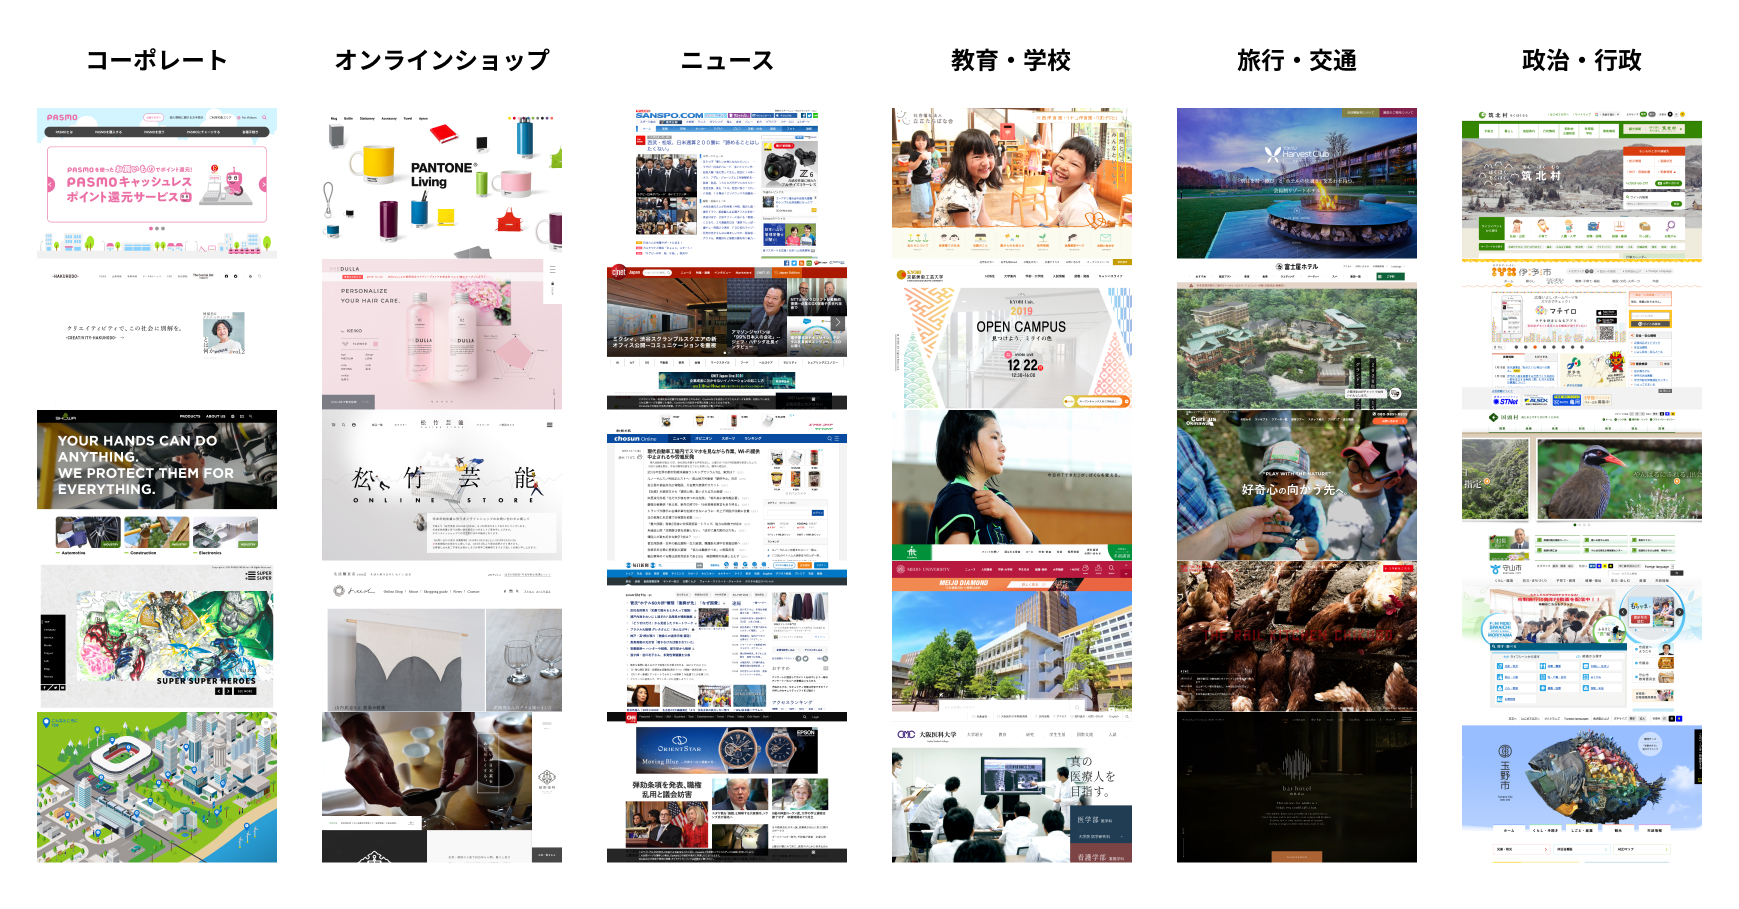
\includegraphics[width=12.5cm]{figures/05_dataset.jpg}
  \caption{データセットに含まれるウェブページの例}
  \label{fig_webpage-dataset}
\end{figure}

\par 収集したウェブサイトは日常で閲覧する多くのサイトをカバーできるように様々な異なるカテゴリから構成されており、被験者が実験中にレイアウトによる視線の偏りが発生することを防ぐことができる。


\subsection{アイトラッカーを使用した視線データ収集}
\par 視線データ収集には19歳から26歳の合計35名(男性:27名、女性:8名)が参加した。被験者は日常でインターネットを使用するネットユーザーでいずれも健常者であった。

\par 視線データ収集はTobii Pro Nano\cite{tobiipronano}を使用して行い、被験者は1920px×1080pxの画面から60cm離れた位置でウェブページを閲覧した。ウェブページのスクリーンショットは画面の中央に最大サイズで表示して視線のデータはTobii Pro Labo\cite{tobiiprolabo}を使用して60Hzのサンプリングレートで記録された。各被験者は正確な視線データを記録するためにレコーディングを始める前にキャリブレーションを行った。その後ウェブデータセットの中からランダムにウェブページが10秒間表示され目的なしの自由状態で閲覧した。ウェブページを閲覧した後5秒間黒い画面が表示され、これらを合計20個のウェブページで実施した。また、各被験者はこれらのセットを休憩を挟んで合計2セット実施した。


\subsection{データ分析}
\par 図\ref{fig_dataset-saliency}で収集したウェブページの視線データの例をヒートマップで示す。ウェブページのレイアウトによって視線が集まる領域は様々で、特に左上から中央付近にかけて視線が集まりやすいことが分かる。また、人物が映る写真が存在する場合、顔付近に注目が集まりやすい傾向があることも分かる。これらの視線座標の傾向を分析するために私たちは特に視線座標との関係性が高いウェブページ固有のレイアウトに着目して第\label{subsec:webdataset}節で作成したウェブデータセットをレイアウトパターンに分類した。なお、レイアウトパターンの選択については既存研究でウェブページのレイアウトパターンを定義しているものが存在しないため、Webデザイン、これからどうなるの?\cite{bookwebdesign}などの書籍やウェブページレイアウトについてまとめられたサイトから既存のウェブページレイアウトをカバーできるように表\ref{table:layoutpattern}に示す合計7パターンに決定した。それぞれのレイアウトパターンに該当するウェブページの例を図\ref{fig_layout_example}に示す。


私たちは収集した視線データセットをランダムに4:1に分類して216個のウェブサイトをオリジナルモデルの学習用に使用し、残りの54個を評価実験用に使用した。

\begin{figure}[H]
  \centering
  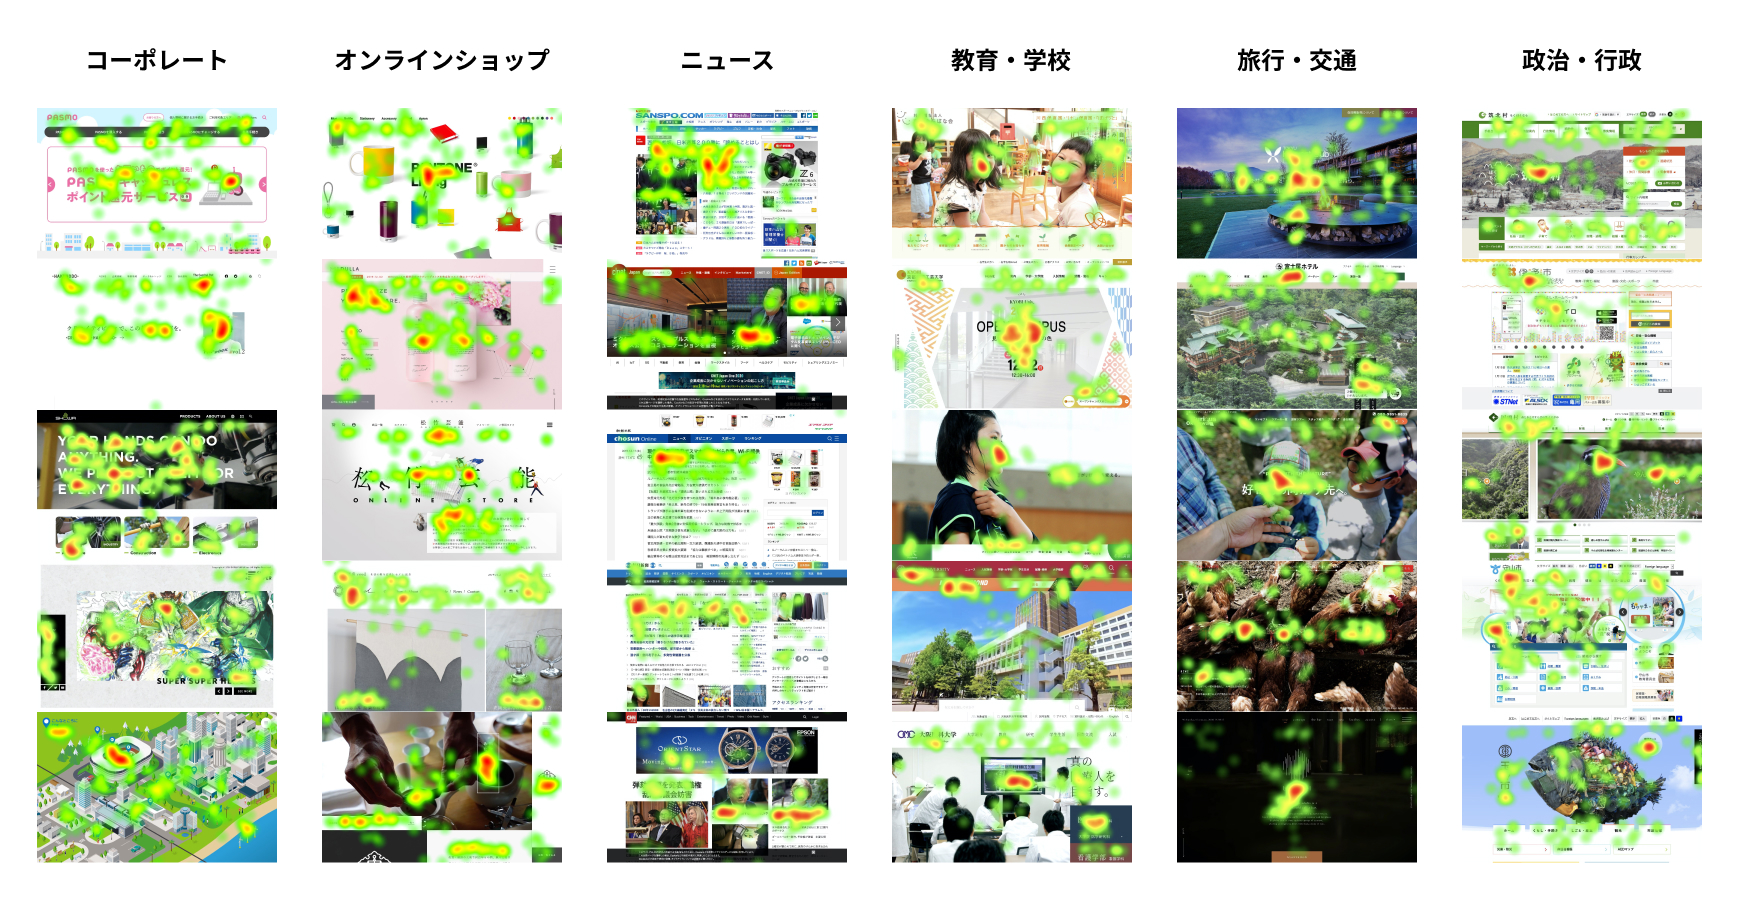
\includegraphics[width=12.5cm]{figures/05_dataset_saliency.jpg}
  \caption{記録した視線データの例}
  \label{fig_dataset-saliency}
\end{figure}

\begin{table}[h]
  \caption{位置情報とサイズを取得するタグの一覧}
  \label{table:layoutpattern}
  \centering
    \begin{tabular}{clll}
    \hline
    パターン名 & 説明 \\
    \hline \hline
    シングルカラム & ページが一列で構成されるレイアウト \\
    2カラム & ページが二列で構成されるレイアウト \\
    3カラム & ページが三列で構成されるレイアウト \\
    4カラム & ページが四列で構成されるレイアウト \\
    カードレイアウト & カードのようなブロック要素が並べられるレイアウト \\
    ブロークングリッド & 要素が画面の様々な位置に散りばめられたモダンデザイン \\
    フルスクリーン & 画面全体にトップビューが広がるモダンデザイン \\
    \hline
  \end{tabular}
\end{table}

\begin{figure}[H]
  \centering
  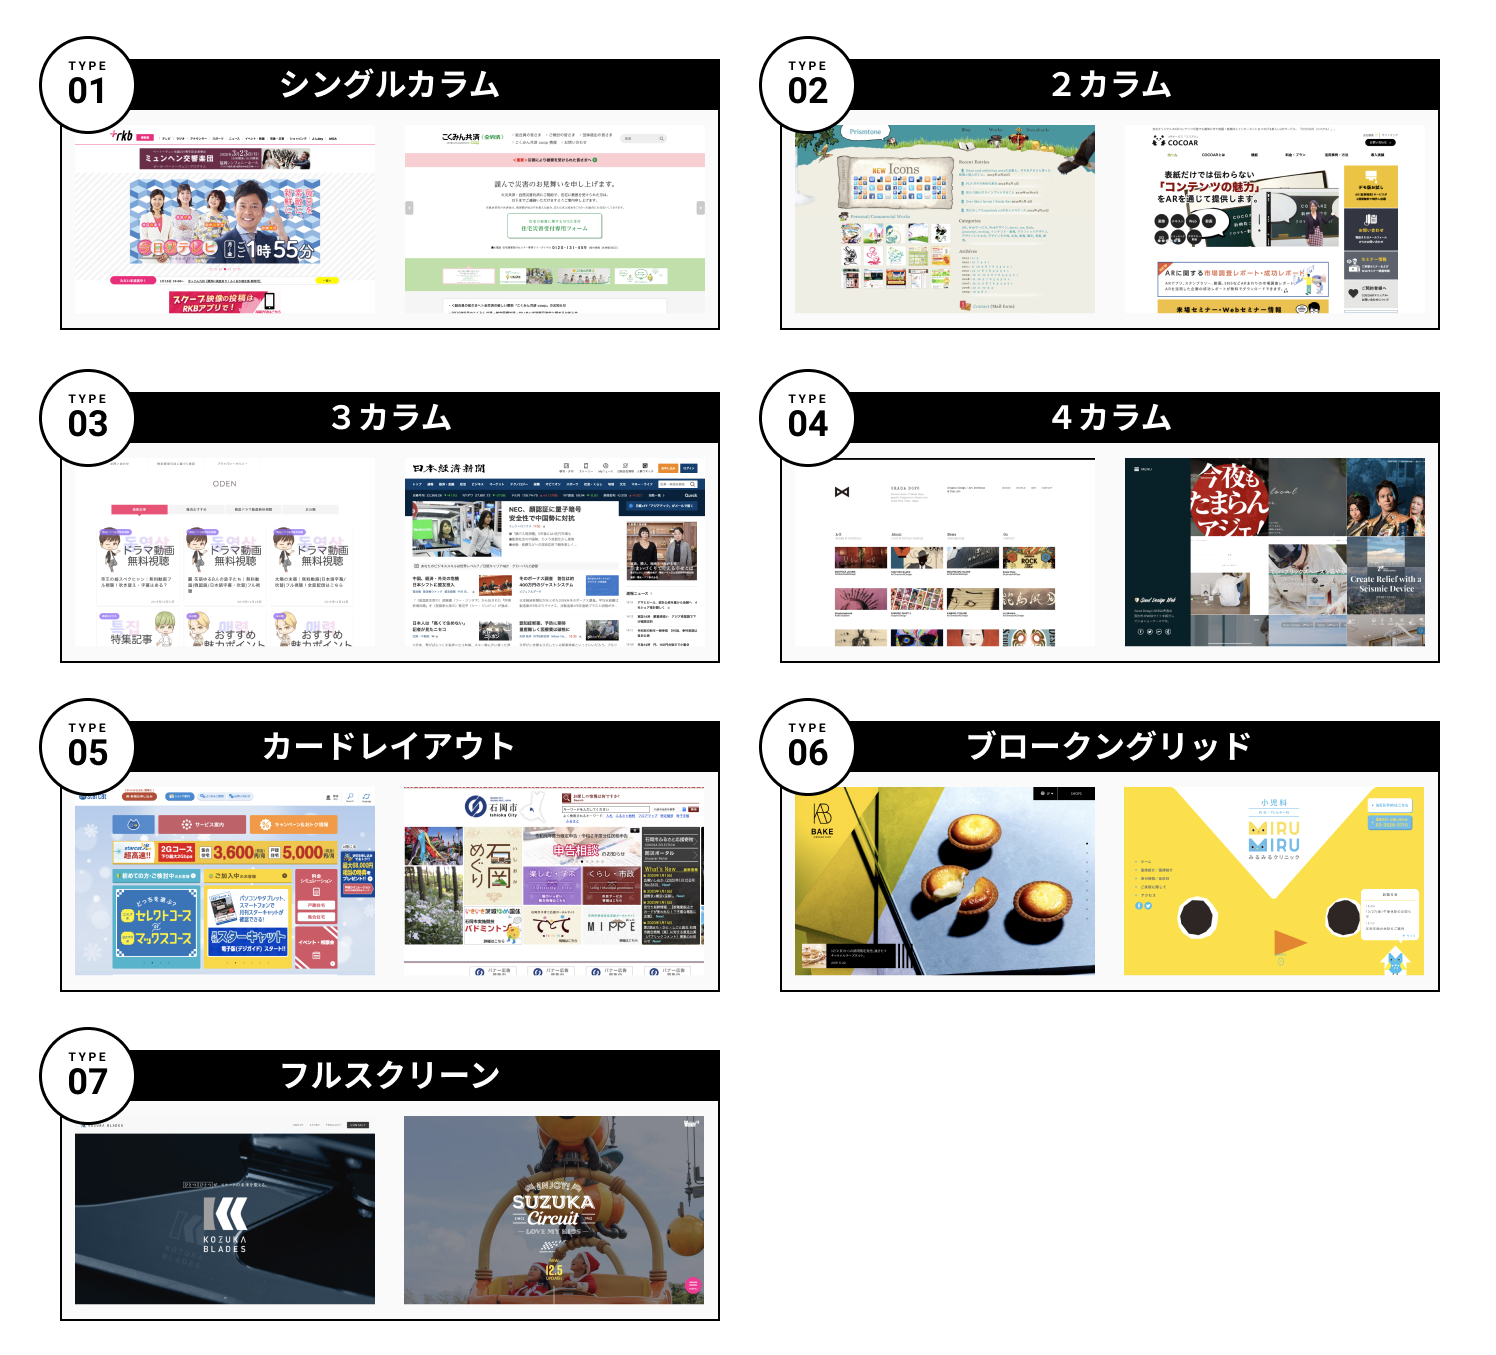
\includegraphics[width=10cm]{figures/05_layout.jpg}
  \caption{各レイアウトパターんに該当するウェブページの例}
  \label{fig_layout_example}
\end{figure}

\begin{figure}[H]
  \centering
  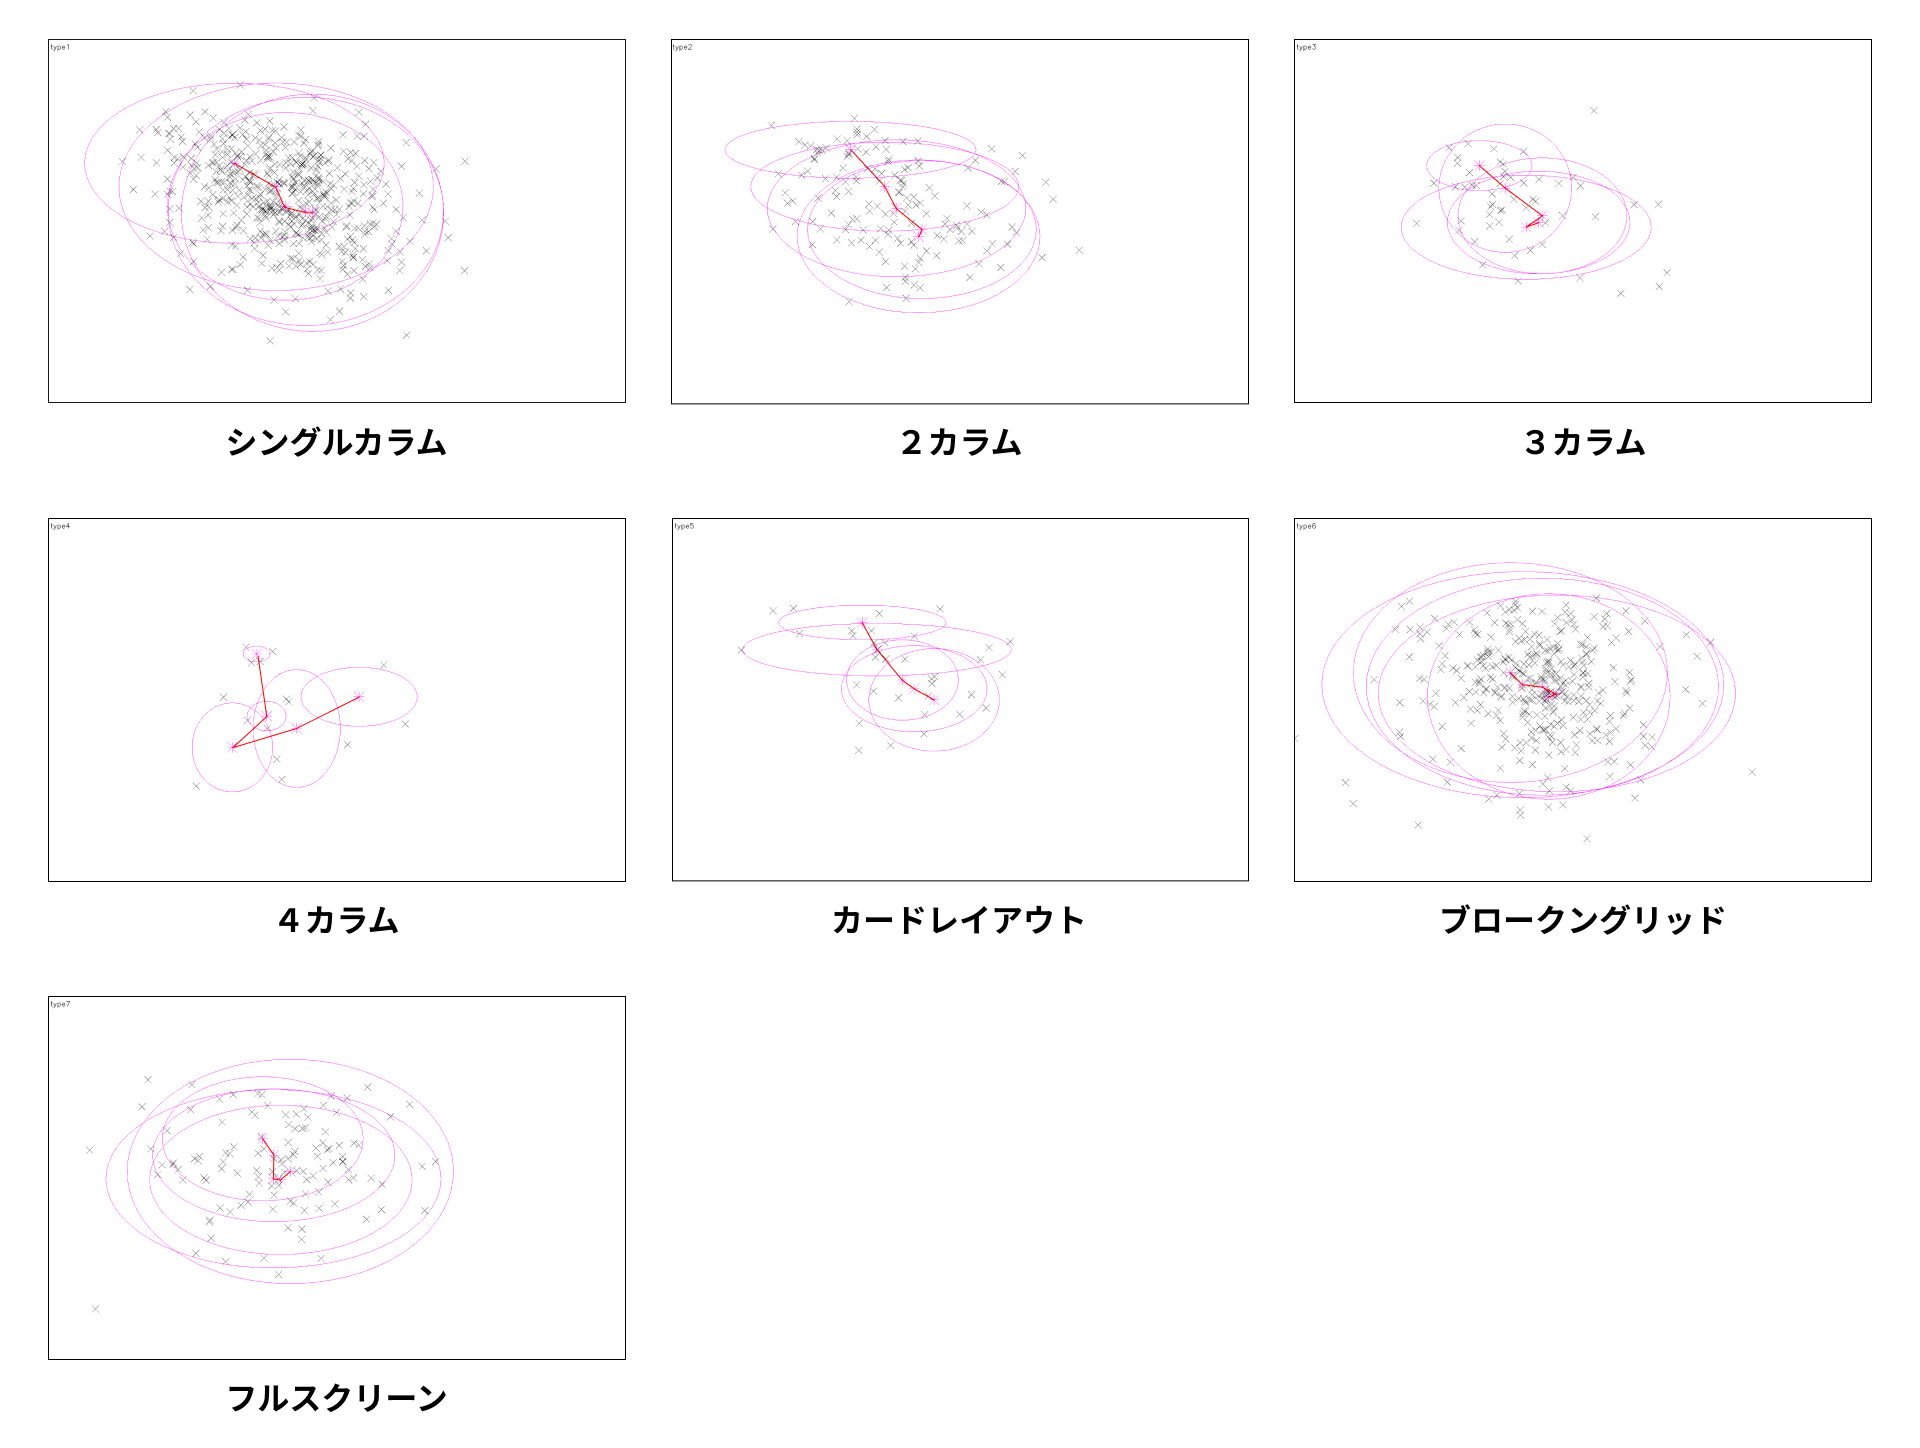
\includegraphics[width=12cm]{figures/05_layout_result.jpg}
  \caption{ウェブページのレイアウト分類結果}
  \label{fig_layout_result}
\end{figure}